\chapter{Simulations cosmologiques}

\newthought{Cet ouvrage est un ouvrage de théorie}. Il s'agit d'exposer les quantités physiques pertinentes, les temps ou échelles caractéristiques importantes à l'évolution et l'établissement des propriétés de l'Univers : à cette fin, nous posons et analysons les équations que nous croyons pertinentes pour extraire ces informations. C'est une tâche qui généralement ne peut se faire que sous certaines hypothèses dont on sait qu'elles ne sont qu'imparfaitement satisfaites dans la réalité. Par exemple, le principe cosmologique\index{principe cosmologique} présuppose une distribution homogène de la matière or nous savons que cela est n'est plus vrai sur des petites échelles \sidenote{on peut mentionner les oscillations baryoniques acoustiques dans le fond diffus ($\lambda < 200$ Mpc comobile) ou bien la présence d'amas de galaxies dans l'Univers actuel ($\lambda < 1$ Mpc comobile)}.  De même, la théorie de l'instabilité gravitationnelle présentée dans le chapitre sur la formation des structures n'est valable que dans le régime des petites perturbations, autorisant une description linéaire de leur croissance : pour autant, nous savons qu'une galaxie présente un contraste de densité $\delta \sim 200$ qui va bien au-delà des limites du régime linéaire. Il existe certes des approches permettant de dépasser le régime des petites perturbations, mais elles nécessitent des conditions précises de symétries par exemple \sidenote{tel le modèle d'effondrement sphérique}.


Pour toutes ces raisons, il est tout un domaine de la cosmologie physique qui vise à développer des outils de simulations numériques\index{simulations numériques} permettant notamment de suivre la structuration de la matière dans des régimes arbitraires de symétries et de non-linéarités. Ces simulations sont essentiellement dédiées à l'étude de la \textit{dynamique} de la matière dans l'Univers en produisant des portions d'Univers synthétiques en évolution depuis les premiers instants jusqu'à nos jours. Elles reproduisent ce que nous pensons être l'histoire complexe de croissance et d'assemblage des structures : en comparant les prédictions de ces outils à la «réalité terrain», il s'agit de tester les lois physiques qui sont utilisées et nos hypothèses sur l'état initial de l'Univers et ses propriétés. Par ailleurs, ces simulations fournissent des histoires de croissances des structures qui peuvent être enrichies de modèles supplémentaires pour explorer des physiques qui ne se limitent pas à la dynamique. Elles sont aussi utilisées à des fins pratiques pour mettre au point des relevés, préparer des observations ou simuler des instruments. Ces outils numériques sont appelés \textit{simulations cosmologiques} et leurs principes les plus importants sont décrits dans ce chapitre.

\begin{figure}[htbp]
	\centering
		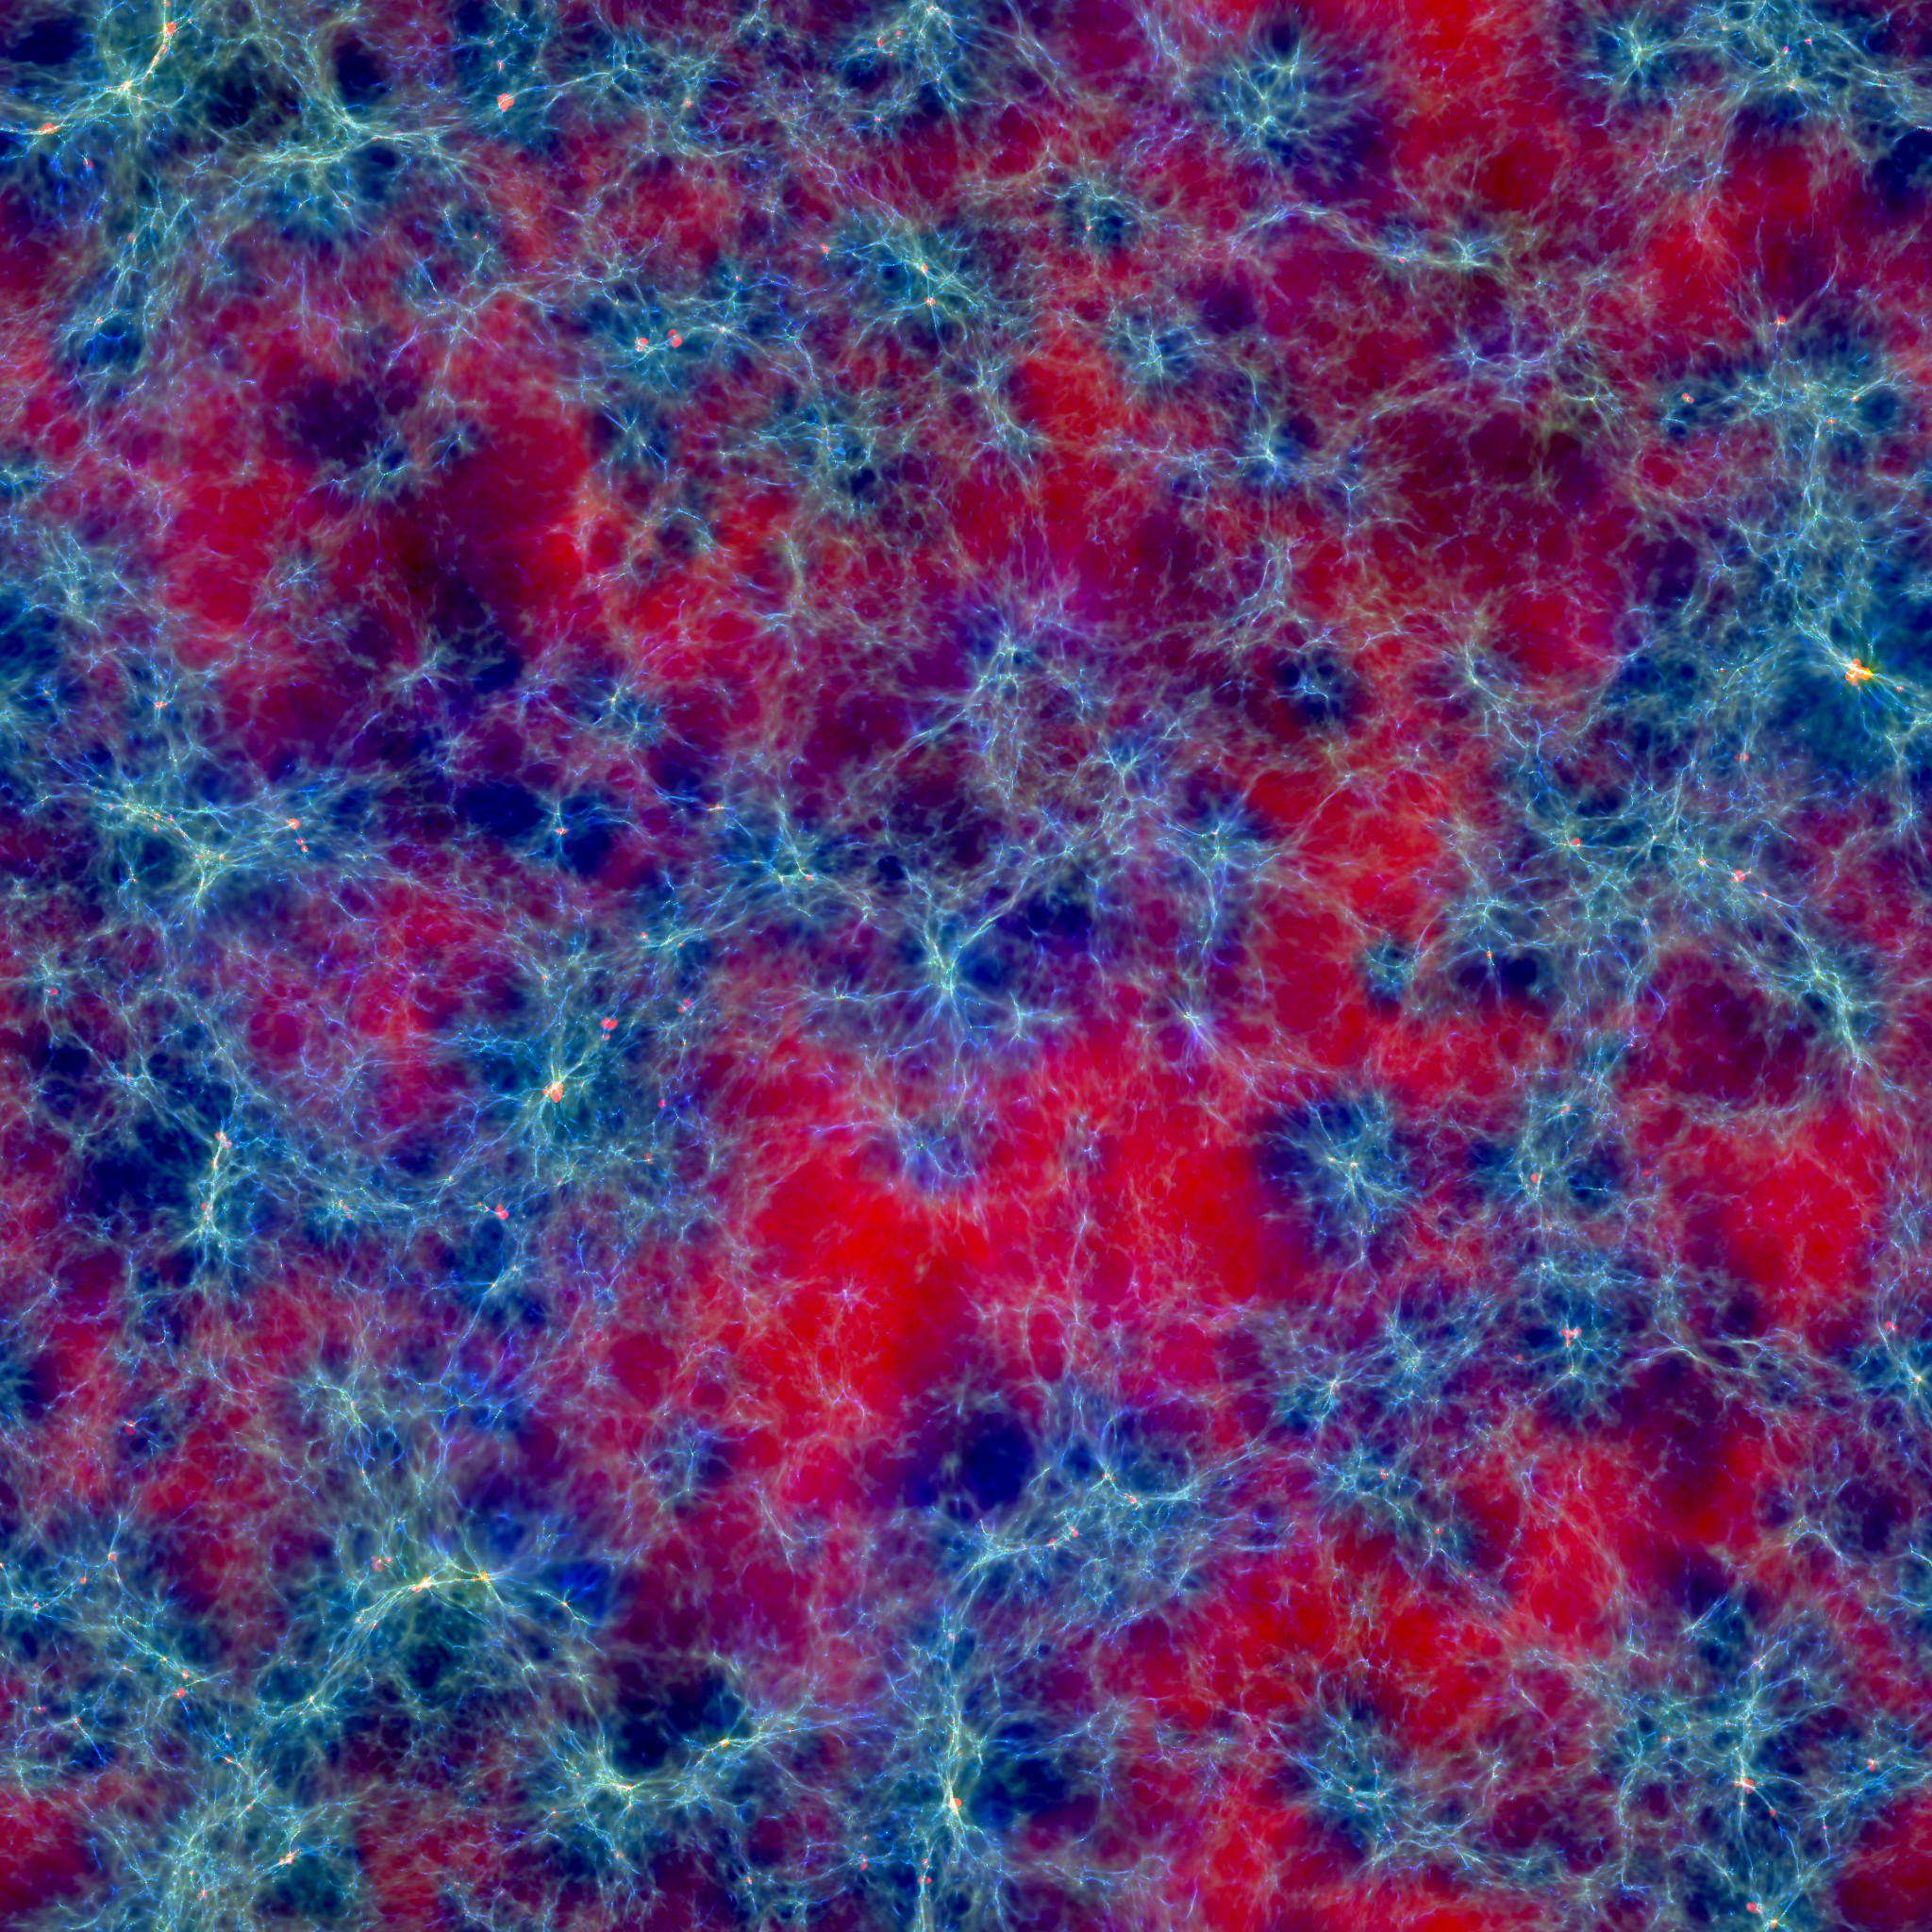
\includegraphics[height=20cm]{figs/simuemma.png}
	\caption[Un exemple de produit de simulation cosmologique]{Un exemple de produit de simulation cosmologique. Cette image montre une prédiction numérique de l'état de l'Univers 1 milliard d'années après le Big-Bang : les structures filamentaires tracent la densité du gaz et le «brouillard» désigne les régions à température élevée ($>20000$ K). L'image fait 90 Mpc de côté.}
	\label{f:simuemma}
\end{figure}

\section{De la discrétisation et de la résolution}
Ces simulations sont produites par des codes informatiques devant tourner sur des ordinateurs. Ces machines possèdent des ressources finies et manipulent des quantités \textit{discrètes}, ce qui est en contradiction avec notre description habituelle du monde qui repose généralement sur une description \textit{continue} : un volume permet une infinité de positions possibles ou bien tous les instants sont accessibles à l'intérieur d'un intervalle temporel donné. Même une quantité à priori dénombrable peut donner l'apparence d'une infinité, tel un nombre de particules qui dans des volumes cosmologiques peut être tout simplement gigantesque. Un traitement informatique implique donc de discrétiser le temps, l'espace, la distribution de matière, etc. pour pouvoir être envisageable.
Par la suite, nous considérons la densité de matière dans l'espace $\delta(\vec x)$ : ce champ scalaire est défini en tout point de l'espace et possède donc une infinité de valeurs possibles tout en étant mesurable dans une infinité de positions possibles. 

\newthought{Une première façon} de segmenter ce champ consiste à l'évaluer à des positions discrètes, par exemple sur une grille\index{simulations numériques!grille} cartésienne de taille de maille $\Delta x$ : cette façon de faire est dite \textit{eulérienne}\index{eulérienne!discrétisation} et permet de réduire le nombre de points où le champ est évalué tout en lui permettant toujours d'accéder à un spectre continu de valeurs en chacun de ces points. Cette méthode introduit en revanche un paramètre de résolution spatiale $\Delta x$ qui va limiter notre capacité à décrire des phénomènes d'échelles caractéristiques proches ou inférieures à cette longueur. On pourra limiter l'influence de ce paramètre de résolution en adoptant par exemple des grilles non cartésiennes, non homogènes ou non statiques, mais on ne pourra jamais la faire disparaître complètement.

\newthought{Une seconde façon} de procéder consiste à découper la matière en quanta souvent appelés \textit{particules}\index{simulations numériques!particules}, qui représente une quantité prédéfinie de matière se déplaçant librement dans l'espace. Cette description est dite \textit{lagrangienne}\index{lagrangienne!discrétisation} et permet d'accéder à tous les points de l'espace de façon continue. En revanche elle introduit également un élément de résolution, en masse cette fois-ci, correspondant à la masse de la particule $m$ : en un point de l'espace, la quantité matière ne pourra augmenter progressivement depuis zéro qu'en «empilant» des particules à cet endroit, d'abord $m$ puis $2m,3m$ etc. Par ailleurs, cette discrétisation en quanta peut introduire du bruit si une quantité de matière donnée n'est représentée que par un faible nombre de particules. Enfin, comme pour la résolution spatiale mentionnée précédemment, cette résolution en masse nous limite dans la description de phénomènes opérant dans des objets de masse inférieure à cette valeur.

\newthought{Concernant le temps,} le même problème se pose: les techniques de résolution approchée d'équations différentielles nécessitent généralement de raisonner sur des durées courtes, par exemple pour satisfaire au mieux des approximations d'ordre linéaire ou de bas ordre. Il faut donc découper les durées d'intérêt en \textit{pas de temps} $\Delta t$ qui à nouveau nous limitent quant à la description de phénomènes plus rapides que cette résolution temporelle. Une simulation numérique tâchera donc de suivre l'évolution de champs discrétisés\index{simulations numériques!discrétisation} sur des grilles (dans une approche eulérienne) ou en particules (dans une approche lagrangienne), en les mettant à jour tous les $\Delta t$ jusqu'à ce que la durée voulue soit couverte. Notons que les 2 approches mentionnées (grille ou particules) possèdent chacune leurs avantages et leurs inconvénients en fonctions des champs considérés et des équations différentielles qui leur sont associés.


\section{Dynamique Non-Collisionelle: Matière noire et étoiles}

Considérons dans un premier temps la composante non collisionnelle de la matière, à savoir la matière noire\index{matière noire} et les étoiles\index{etoiles@étoiles}. Dans la plupart des cas, une simulation cosmologique va décrire ces composantes sous forme de particules possédant une masse $m$, une position $\vec x_i$ et une vitesse $\vec v_i$ ( $i$ désignant la particule parmi N autres). La masse ne varie pas, tandis que positions et vitesses subissent des mises à jour régulières via la résolution du principe fondamental de la dynamique\index{principe fondamental de la dynamique} :
\begin{equation}
\frac{d \vec v_i}{dt}=\frac{1}{m} \vec{F}(\vec x_i)
\end{equation}
où $\vec{F}(\vec x_i)$ désigne la résultante des forces à la position $\vec x_i$. Pour une composante non collisionelle, cette résultante est uniquement le fruit de la force de gravitation. Un schéma de mise à jour simple peut prendre pour point de départ la discrétisation suivante \sidenote{par la suite on négligera la forme vectorielle des positions et vitesses en se ramenant à un problème 1D. La généralisation à 3D ne posant pas de difficultés.}:
\begin{equation}
\frac{v_i^{p+1}-v_i^{p}}{\Delta t}=\frac{1}{m} {F}(x_i^p)
\end{equation}
et permet d'évaluer la vitesse $v_i^{p+1}$ à l'instant $t^{p+1}=t^p+\Delta t$ comme suit:
\begin{equation}
v_i^{p+1}=v_i^{p}+\frac{\Delta t}{m} {F}(x_i^p).
\end{equation}
Par ailleurs, ayant $dx/dt=v$, on obtient aisément la formule de la mise à jour de la position:
\begin{equation}
x^{p+1}_i=x^{p}_i+\Delta t v_i^{p+1}.
\end{equation}
Ce schéma d'avancement\index{schéma d'avancement} simple est l'une des formes du \textit{schéma d'Euler}\index{schéma d'Euler} : s'il a le mérite de la simplicité, à l'usage il présente des inconvénients en termes de stabilité ou de précision qui nécessitent de manipuler des pas de temps $\Delta t$ particulièrement courts. D'autres schémas plus complexes existent, garantissant une meilleure stabilité ou précision, par exemple le \textit{leapfrog}\index{leapfrog}\sidenote{une traduction possible serait «saute-mouton»}
\begin{eqnarray}
v_i^{p+1/2}&=&v_i^{p-1/2}+\frac{\Delta t}{m} {F}(x_i^p)\\
x^{p+1}_i&=&x^{p}_i+\Delta t v_i^{p+1/2}
\end{eqnarray}
où l'on voit que vitesse et position sont évaluées de façon désynchronisée avec un décalage de $\Delta t/2$. L'un des mérites de cette méthode est son invariance par renversement du temps \sidenote{on parle de schéma symplectique\index{schéma symplectique}} : en appliquant une mise à jour de $-\Delta t$ le leapfrog permet de retrouver la position $x^p$ à partir de $x^{p+1}$. Le schéma d'Euler ne possède pas la même propriété à cause du terme de force qui passe de ${F}(x_i^p)$ à  ${F}(x_i^{p+1})$ selon qu'on aille dans un sens ou l'autre. 

\newthought{La dernière inconnue} est l'expression de la force en tout point de l'espace ${F}(x_i^p)$. Plusieurs techniques ont été développées depuis les années 70, mais peuvent être rapidement regroupées en 2 familles. La première repose sur un principe de sommation\index{N-Corps!direct}. On dispose des positions $x_i$ de toutes les $N$ particules, on peut donc calculer la force appliquée sur la particule $j$ en sommant toutes les forces individuelles créées par les particules $i$ qui s'appliquent dessus \sidenote{on suppose que toutes les particules sont de masse $m$. $r_{ij}$ désigne la distance entre les particules i et j, tandis que $\vec e_ij $ désigne le vecteur unitaire les reliant} :
\begin{equation}
\vec F_j=-Gm^2\sum_{i\neq j} ^N\frac{1}{r_{ij}^2}\vec e_{ij}. 
\end{equation}
Cette méthode de sommation directe\index{sommation directe} est simple à mettre en place et est rigoureusement exacte, toutefois elle est extrêmement coûteuse puisqu'elle nécessite d'évaluer $N(N-1)/2 \sim N^2$ interactions : si l'on décide de multiplier par 10 le nombre de particules (pour gagner en résolution en masse et étudier de plus petits objets par exemple), cela implique 100 fois plus de calculs. Ce type de dépendance en $N^2$ pour le coût de calcul est tout simplement insoutenable en pratique. Pour cette raison il existe des techniques qui permettent d'accélérer ce type de sommation\index{sommation} par exemple en subdivisant hiérarchiquement l'espace suivant une configuration arborescente\index{N-Corps!arbre}\sidenote{on parle usuellement de \textit{tree-code} ou code en arbre}. Dans ces approches, une région distante (et donc peu influente) est vue avec peu de détails en regroupant les particules qui s'y trouve en «macro-particules» moins nombreuses, ce qui réduit le cout informatique de la sommation : on peut montrer que le nombre d'interactions suit une loi en $N\log N$, bien plus soutenable. Pour finir, remarquons que la formule de sommation peut diverger si certaines particules sont trop proches les unes des autres avec $r_{ij}\rightarrow 0$ : en pratique, il est d'usage de lisser la force de gravitation sur une échelle $\epsilon$. Par exemple on peut écrire
\begin{equation}
\vec F_j=-Gm^2\sum_{i\neq j} ^N\frac{1}{r_{ij}^2+\epsilon^2}\vec e_ij. 
\end{equation}
où $\epsilon$ empêche la force de diverger aux faibles séparations, mais au prix d'une réduction de la résolution spatiale : aux échelles de l'ordre du lissage, la force n'est plus correctement décrite.

La seconde famille de méthode pour l'évaluation de la force passe par l'estimation du champ potentiel gravitationnel $\phi(\vec x)$ sur une grille (très généralement) cartésienne\index{simulations numériques!grille}. Force et potentiel\index{potentiel gravitationnel} dérivent l'un de l'autre :
\begin{equation}
\vec F (\vec x) =-\nabla \phi(\vec x)
\end{equation}
tandis que le potentiel peut être évalué en résolvant l'équation de Poisson\index{équation de Poisson@equation de Poisson} à partir du champ de la densité massique $\rho(\vec x)$:
\begin{equation}
\Delta \phi(\vec x) = 4\pi G \rho(\vec x).
\label{e:poissPM}
\end{equation}
Connaissant la position $\vec x_i$ de toutes les particules, on peut évaluer la densité  $\rho(\vec x)$ en tous les points d'une grille\sidenote{en pratique il s'agit de calculer l'histogramme 3D des positions de ces particules} et donc le potentiel $\phi(\vec x)$ puis la force $\vec F(\vec x)$. Connaissant la force en tous les points d'une grille, on peut alors l'interpoler aux positions désirées à savoir les positions $\vec x_i$ de toutes les particules.
\begin{figure}[htbp]
	\centering
		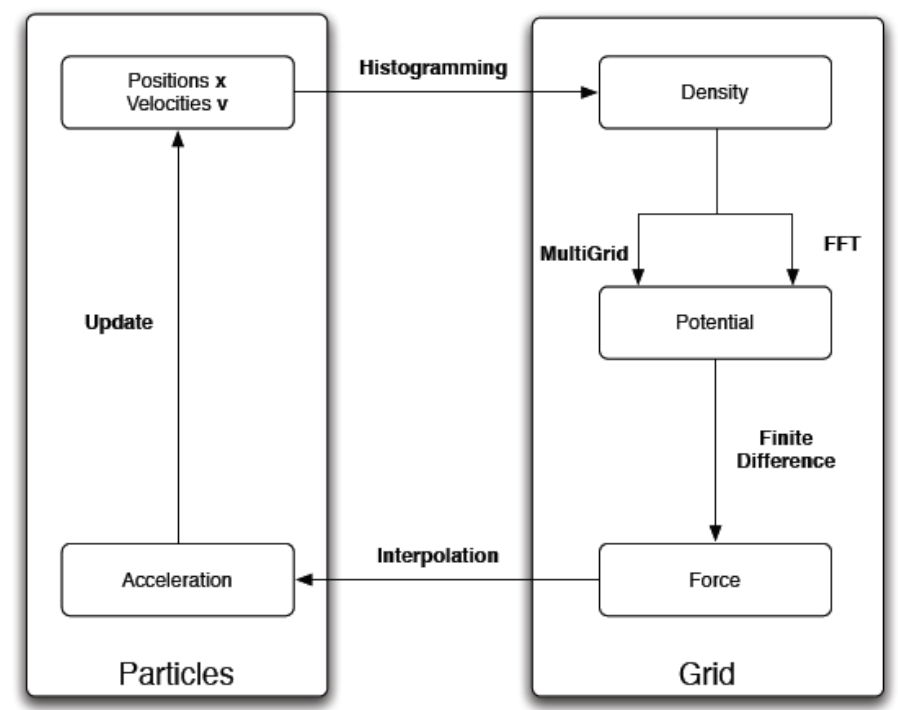
\includegraphics[height=6cm]{figs/PM.png}
	\caption[Schématique de la méthode de calcul des forces sur grilles.]{Schématique de la méthode de calcul des forces sur grilles. Notez la nature hybride du schéma qui fait intervenir une description en termes de particules (ou lagrangienne à gauche) et une description en termes de champs sur une grille (ou eulérienne à droite)}
	\label{f:PM}
\end{figure}
Pourquoi se donner tant d'efforts pour évaluer la force ou le potentiel de cette façon ? La réponse réside dans la résolution de l'équation de Poisson\index{equation@équations!Poisson} (éq. \ref{e:poissPM}). Cette équation est fondamentalement une équation de diffusion, et nombre de méthodes ont été développées pour la résoudre efficacement et rapidement dans de nombreux contextes. Par exemple, prenons la transformée de Fourier (TF) de l'équation de Poisson et nous obtenons aisément\sidenote{voir aussi le chapitre dédié à la matière noire} : 
\begin{equation}
\tilde \phi(\vec k)\sim -\frac{\tilde \rho(\vec k)}{k^2}.
\end{equation} 
Si nous avons une façon simple d'évaluer les transformées de Fourier de champs connus sur une grille, il suffit d'appliquer l'équation algébrique triviale précédente pour trouver le potentiel à partir de la TF de la densité et du potentiel. Il s'avère qu'il existe des techniques de \textit{transformées de Fourier rapide}\index{transformée de Fourier} ou FFT qui ont été développées durant des décennies à des fins de traitement du signal et qui donc peuvent être facilement reprises. 

Par ailleurs, il existe aussi des méthodes dites de «relaxation»\index{méthodes de relaxation} qui permettent de résoudre l'équation de Poisson : si l’on examine cette dernière, on peut considérer qu'elle n'est qu'un cas particulier de l'équation de diffusion
\begin{equation}
\frac{\partial \phi(\vec x,t)}{\partial t}+\Delta \phi(\vec x,t) = 4\pi G \rho(\vec x)
\end{equation}
dans le régime \textit{stationnaire}, avec $\frac{\partial \phi(\vec x,t)}{\partial t}\rightarrow 0$. En cherchant cette solution stationnaire, on peut trouver une solution de l'équation de Poisson. Une version de cette équation en différences finies donne \sidenote{ici $i$ désigne une cellule donc une position dans la grille tandis que $p$ désigne une estimation du potentiel}:
\begin{equation}
\frac{\phi^{p+1}_i-\phi^{p}_i}{\Delta t}+\frac{\phi^{p}_{i+1}-\phi^{p}_{i-1}}{\Delta x^2}=4\pi G\rho^{p}_i
\end{equation}
que l'on peut réarranger sous la forme d'une équation de \textit{relaxation}\index{relaxation}:
\begin{equation}
\phi^{p+1}_i=\phi^{p}_i+4\pi G\rho^{p}_i-\frac{\phi^{p}_{i+1}-\phi^{p}_{i-1}}{\Delta x^2}\Delta t.
\end{equation}
En se donnant une estimation du potentiel $\phi^{p}_i$ à une itération $p$ et en l'utilisant dans cette relation de relaxation, on s'approche en principe d'une estimation encore meilleure $\phi^{p+1}_i$. D'itération en itération, on peut ainsi converger vers une solution du potentiel : notons que l'on utilise un pas de temps \textit{fictif} $\Delta t$ dont on peut montrer qu'une convergence optimale est obtenue pour $\Delta t\sim \Delta x^2/2$. La méthode décrite ici est la plus simple de toutes les méthodes de relaxation \sidenote{c'est la méthode de \textit{Jacobi}\index{méthode de Jacobi}}: il en existe d'autres, plus stables, plus efficaces dont les méthodes dites \textit{multigrilles} qui cherchent à faire converger les différentes échelles du potentiel de façon séparée et optimale. Comparées aux méthodes à base de FFT, elles sont plus versatiles\sidenote[][-2cm]{on peut aussi les utiliser pour des versions modifiées de l'équation de Poisson ou sur des grilles non cartésiennes} et légèrement moins rapides.

Que ce soit grâce à la FFT ou aux méthodes de relaxation, on dispose de moyens extrêmement rapides de résolution de l'équation de Poisson : en revanche, l'utilisation d'une grille implique que le champ de gravitation n'est décrit qu'au mieux sur une échelle de la taille d'une cellule de la grille. Une telle échelle de coupure est inexistante à priori dans les méthodes de sommation qui permettent donc un suivi plus précis et à plus petites échelles des effondrements par exemple. L’utilisation d'un lissage $\epsilon$ dans les méthodes de sommation introduit certes une résolution limite, mais ce lissage est généralement bien plus petit que la taille d'une cellule (environ 10 fois plus petit en pratique). De fait, on n'hésite pas parfois à combiner les méthodes de sommation et celles de type grille pour bénéficier de leurs avantages respectifs.

Pour finir, considérons rapidement la différence entre particules de matière noire\index{matière noire} et étoiles\index{etoiles@étoiles}, qui toutes deux sont l'objet de la dynamique non-collisionnelle. Dans les 2 cas, les méthodes exposées ici sont appliquées de façon identique, les deux espèces diffèrent en ce que leurs membres n'évoluent pas de la même manière. Les particules de matières noires n'évoluent pas, leur masse individuelle reste constante, leur nombre initial fixe la quantité de matière noire et il n'a pas d'annihilation ni de création de telles particules. Les étoiles évoluent: elles doivent apparaître lorsque les conditions s'y prêtent et elles peuvent voir leur masse évoluer : en effet, une particule «stellaire» constitue en pratique un amas stellaire  de plusieurs centaines d'étoiles à plusieurs millions de masses solaires. Elles représentent donc davantage une population qu'une étoile individuelle en tant que telle : lorsque les étoiles les plus massives de ces amas explosent en supernovæ\index{supernovæ}, la masse est rendue au milieu interstellaire au bout de quelques millions d'années et numériquement cela peut correspondre à une masse variable de particule. Notons toutefois qu'il existe toujours au sein de ces particules stellaires une composante «étoile de faible masse» à durée vie supérieure au temps de Hubble: de façon générale une particule stellaire voit sa masse diminuer, mais ne peut complètement disparaître du fait de cette population à grande durée de vie.

\section{Hydrodynamique}
\newthought{En contrepoint} à la dynamique non-collisionnelle, les codes de simulations numériques peuvent également suivre la dynamique du gaz\index{hydrodynamique} présent dans l'Univers. Ces baryons ne représentent certes que $\sim 15\%$ de la matière disponible, mais ils sont observables ou bien sont à l'origine des étoiles qui sont également observables : par conséquent, ils permettent une comparaison plus directe des résultats simulés aux observations. Par ailleurs au centre des galaxies, le gaz peut être dominant et sa dynamique est suffisamment différente de celle de la matière noire et des étoiles pour devoir être modélisée indépendamment.

\newthought{Le jeu d'équation} à résoudre est connu, ce sont les équations d'Euler\index{equation@équations!Euler}\sidenote{représentées ici à 1D. On y distingue l'équation de la conservation de la masse et de l'impulsion. $\rho(x,t)$ désigne la densité de gaz, $v(x,t)$ sa vitesse, $P(x,t)$ sa pression\index{pression} et $\phi(x,t)$ le potentiel gravitationnel.}:
\begin{eqnarray}
\frac{\partial \rho}{\partial t}+\frac{(\partial \rho v)}{\partial x}&=&0\\
\frac{\partial v}{\partial t} + v \frac{\partial v}{\partial x}&=&-\frac{1}{\rho}\frac{\partial P}{\partial x}-\frac{\partial \phi}{\partial x}
\end{eqnarray}
La première équation indique que la densité ne varie que sous l'effet du flux de masse ($\frac{(\partial \rho v)}{\partial x}$) tandis que la seconde indique que l'impulsion varie sous l'effet du flux de moment ($ v \frac{\partial v}{\partial x}$) et des forces de pression ($\frac{\partial P}{\partial x}$)  et de gravitation ($\frac{\partial \phi}{\partial x}$) \sidenote{il s'agit juste d'une formulation alternative du principe fondamental de la dynamique}.

Ces équations peuvent être toutes deux écrites sous une forme \textit{conservative}\index{equation@équation de conservation}
\begin{eqnarray}
\frac{\partial \rho}{\partial t}+\frac{(\partial \rho v)}{\partial x}&=&0\\
\frac{\partial \rho v}{\partial t}+\frac{(\partial \rho v v)}{\partial x}&=&-\frac{\partial P}{\partial x}-\frac{\partial \phi}{\partial x}\\
\frac{\partial E}{\partial t}+\frac{(\partial E v)}{\partial x}&=&-v \frac{\partial P}{\partial x}-v\frac{\partial \phi}{\partial x}
\end{eqnarray}
auxquelles nous avons ajouté l'équation de conservation\index{equation@équations!conservation} de l'énergie $E$. Ces 3 équations suivent une structure similaire, typique d'équations de conservation d'une quantité $A$ avec un terme source\index{terme source}
\begin{equation}
\frac{\partial A}{\partial t}+\frac{\partial F(A)}{\partial x}=S(A).
\label{e:cons}
\end{equation}
Dans les 3 cas, une quantité $A$ est modifiée sous l'effet d'un flux $F(A)$, qui déplace la quantité en question, et d'un terme source qui modifie $A$ sans déplacement. Dans le cas de la densité, ce terme source est strictement nul ce qui indique une conservation stricte de la masse, dans le cas de l'impulsion, ce terme source est constitué des forces qui s'exercent sur le fluide et dans le cas de l'énergie il est finalement constitué du travail de ces mêmes forces.

La façon la «plus naturelle» de résoudre des équations du type d’ Éq. \ref{e:cons} est de considérer un volume fini\index{volumes finis}, comme celui d'une cellule cubique et de mesurer les flux des quantités conservées (densité, impulsion et énergie) au travers des faces de cette cellule. Intuitivement, le flux mesuré au travers d'une face dépend des valeurs physiques de part et d'autre de cette face : la procédure qui permet de trouver le flux de $A$ connaissant $A$ de part et d'autre de l'interface s'appelle une \textit{résolution de problème de Riemann}\index{problème de Riemann}.

 Il existe nombre de façons de résoudre un problème de Riemann, avec des niveaux d'approximations plus ou moins importants. Soit par exemple $F(A_{i+1/2})$, le flux existant entre 2 cellules successives $i$ et $i+1$ : résoudre le problème de Riemann revient à trouver la fonction $\mathcal R$ telle que
 \begin{equation}
 A_{i+1/2}=\mathcal{R}(A_i, A_{i+1/2}).
 \end{equation}
 Une façon simple de procéder revient à comparer les «vents» dans les cellules adjacentes en comparant leurs vitesses: si $v_i>v_{i+1}$ le vent vient de la cellule $i$ et l’on peut considérer que la valeur de $A$ à l'interface est dominée par $A_i$. Cette procédure dite \textit{upwind} va par exemple assigner:
  \begin{equation}
 A_{i+1/2}=\mathcal{R}(A_i, A_{i+1/2})\sim A_i
 \end{equation}
 et donc $F(A_{i+1/2})\sim F(A_{i})$. On peut toutefois montrer que ce type de schéma est soit extrêmement diffusif soit particulièrement instable et il existe toute une littérature de schémas de plus haut niveau, plus ou moins adaptés en fonction du problème que l'on cherche à résoudre.
 
 Connaissant le flux\index{flux} en $i-1/2$ et $i+1/2$, la quantité $A$ peut être mise à jour par le même type de différence finie que celle utilisée précédemment pour le déplacement de particule non collisionelle :
 \begin{equation}
 \frac{A_i^{^p+1}-A_i^p}{\Delta t}=-\frac{F(A_{i+1/2}^p)-F(A_{i-1/2}^p)}{\Delta X}+S(A_i^p)
 \end{equation}
 ou bien
 \begin{equation}
 A_i^{^p+1}=A_i^p-\Delta t \frac{F(A_{i+1/2}^p)-F(A_{i-1/2}^p)}{\Delta X}+\Delta t S(A_i^p).
 \end{equation}
Notez que cette mise à jour à l'instant $p+1$ ne nécessite la connaissance que des données à l'instant $p$ et tous les termes du membre de droite sont évalués à cet instant. Cette approche est dite \textit{explicite}\index{schéma explicite} et n'est que conditionnellement stable. Si le pas de temps $\Delta t$ est trop important, une amplification des erreurs s'opère et la stabilité n'est garantie que si la condition de Courant est satisfaite :
\begin{equation}
\frac{\Delta x}{ \Delta t}> v.
\end{equation}
Cette équation traduit que la vitesse numérique, la vitesse de mise à jour, doit être supérieure à la vitesse typique du processus physique que l'on cherche à reproduire : pour une résolution spatiale $\Delta x$ donnée cela équivaut à mettre une limite supérieure au pas de temps $\Delta t$ choisi \sidenote{Notons que la même chose existe pour les particules de la partie précédente. Si l'on souhaite qu'une particule ne parcoure pas une trop grande distance durant un pas de temps, il faut limiter ce dernier.} Notons qu'il existe aussi une approche dite \textit{implicite}\index{schéma implicite} où tous les termes de mise à jour sont exprimés à l'instant $p+1$ : toutefois, ces termes sont inconnus au moment du calcul et la mise à jour implique dès lors un problème typique d'inversion, souvent compliqué, en lieu et place de la simple expression algébrique obtenue ici. En revanche, l'approche implicite est généralement inconditionnellement stable, ce qui permet l'utilisation de pas de temps plus grands pour simuler un problème donné.

\newthought{Une autre méthode populaire} existe pour traiter les équations hydrodynamiques et qui repose sur une description particulaire des éléments de fluides. Nommée \textit{SPH} (pour \textit{smoothed particle hydrodynamics})\index{SPH} elle repose sur l'utilisation de particules d'extension finie et non nulle. Cette extension est formalisée par un noyau dont la valeur dépend de la distance au centre de la particule, $W(|x-x_p|)$, valeur qui tend vers zéro au-delà d'une certaine \textit{distance de lissage}. Ce noyau fait office de poids et toute quantité intensive (densité, moment, énergie...) associée à une particule s'obtient en additionnant les contributions pondérées de ses $i$ voisines:
\begin{equation}
A=\sum_i m_i \frac{A_i}{\rho_i} W(|x_i-x_p|).
\end{equation} 
Cette somme se fait généralement sur un nombre de particules voisines prédéterminé : si la matière est dense, les distances impliquées seront courtes tandis qu'un état diffus implique naturellement une sommation sur de plus grandes distances.
 
L'intérêt de cette méthode est sa simplicité : par exemple toute dérivée spatiale de $A$ se propage linéairement au noyau de pondération, dont la dérivée est généralement simple et connue. De plus, cette description sous forme de particule n'implique pas de géométrie d'échantillonnage à priori, au contraire d'une grille qui fixe d'emblée des directions ou des points de mesures privilégiés. Les particules de fluides se déplacent librement et peuvent par exemple sur-échantillonner les régions denses ou sous-échantillonner les régions vides : par rapport à une grille, on a ainsi un échantillonnage de l'espace au plus près des contrastes de densité. Son inconvénient majeur est sa plus grande diffusivité comparée aux meilleures formulations sur grille : dans ses versions les plus communes, la méthode SPH ne parvient pas à capturer certains types de chocs ou de discontinuités et ne lui permet pas de reproduire certaines instabilités hydrodynamiques standard. 

\begin{figure}[htbp]
	\centering
		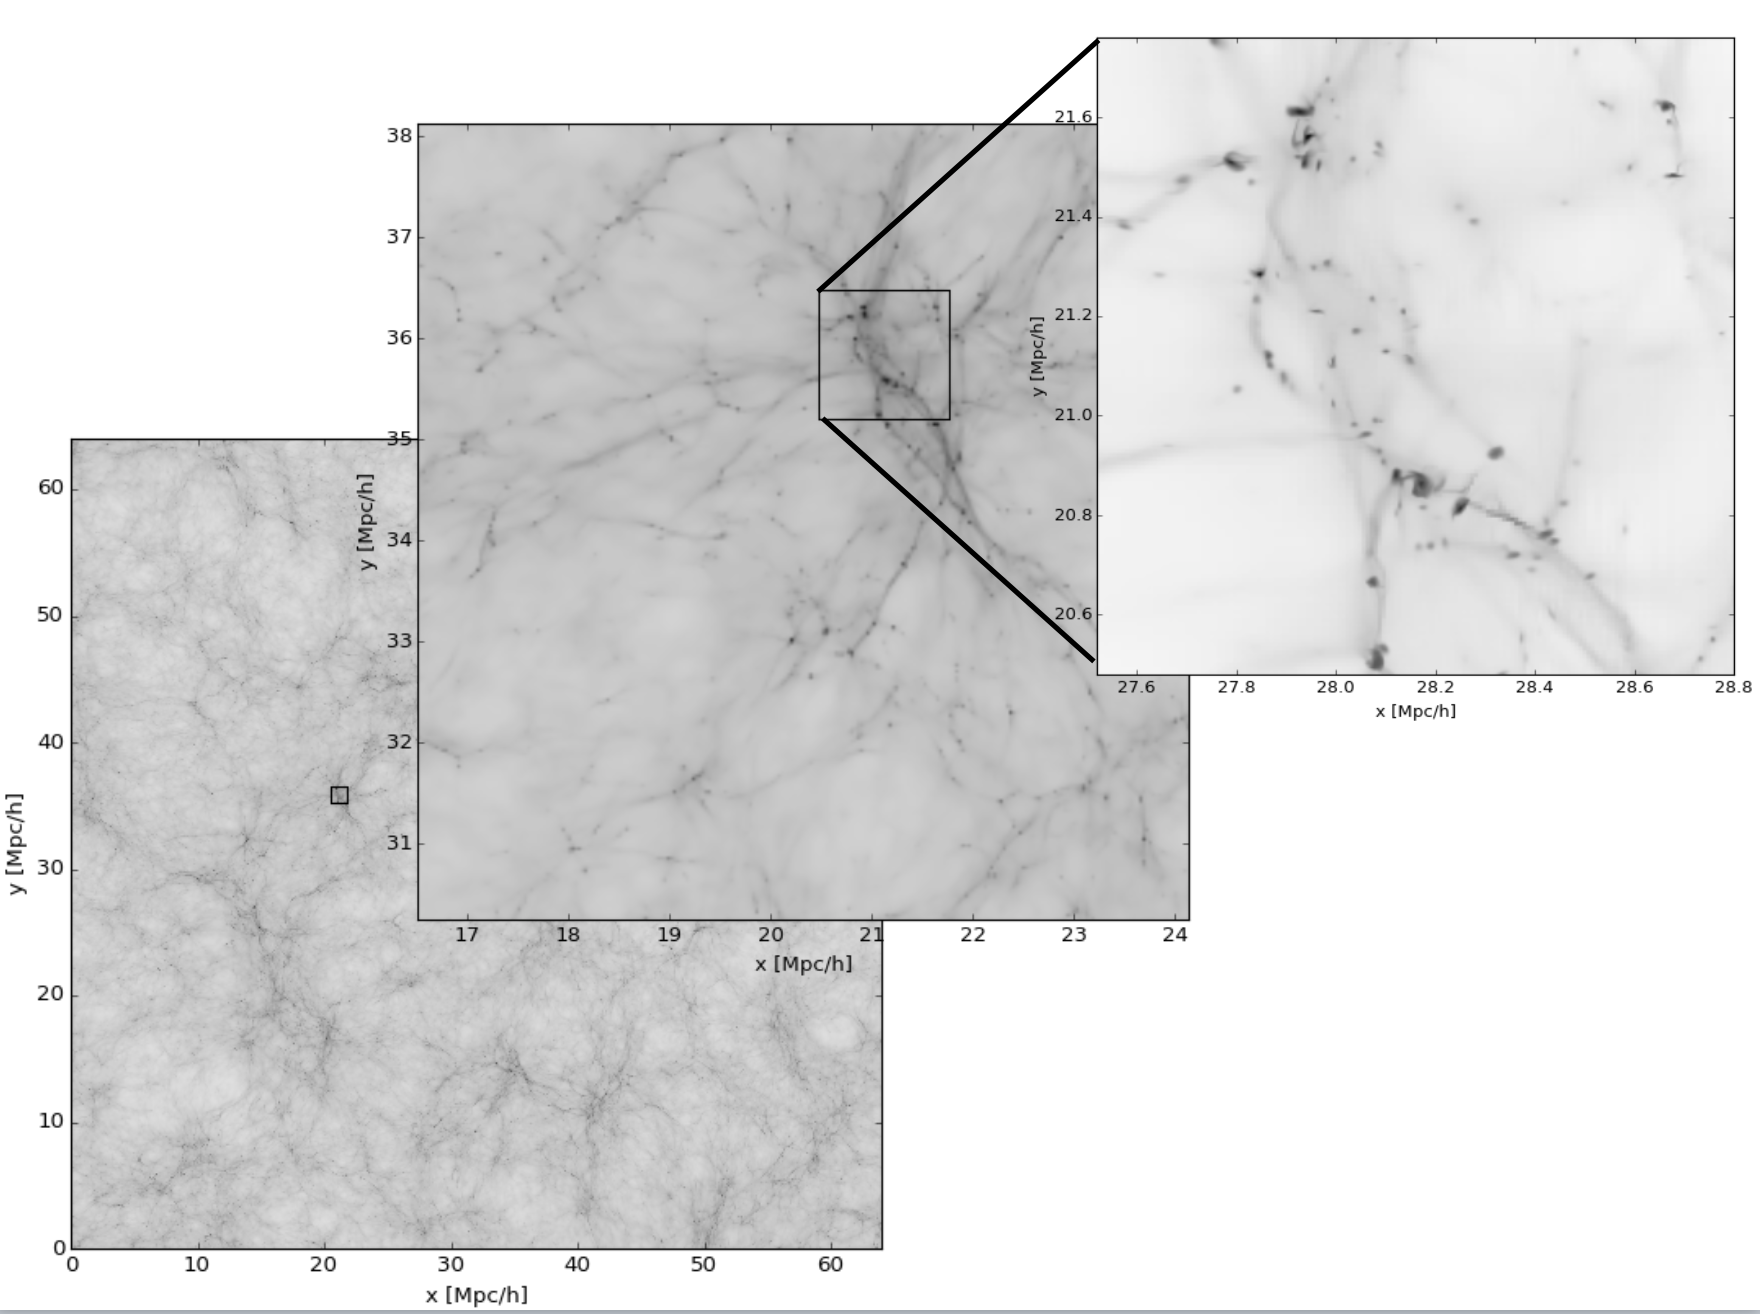
\includegraphics[height=12cm]{figs/zoom.png}
	\caption[Exemple de dynamique dans une simulation hydrodynamique avec refroidissement.]{Exemple de dynamique dans une simulation hydrodynamique avec refroidissement. L'image de droite représente la distribution de gaz dans les 2 cadres de gauches. On note la présence de disques gazeux en rotation créés par le gaz effondré sous l'effet du refroidissement.}
	\label{f:zoom}
\end{figure}


\section{Processus physico-chimiques}
Comme expliqué dans la partie dédiée à la formation des structures, le gaz cosmique ne peut s'organiser sous la forme de galaxies que si ce dernier peut évacuer de l'énergie via des processus de refroidissement\index{refroidissement}. L'équation qui régit l'évolution de l'énergie interne\index{energie@énergie interne} est\sidenote[][-2cm]{$e$ désigne l'énergie interne du gaz tandis que $H$ et $\Lambda$ désignent respectivement les fonctions de chauffage et de refroidissement} :
\begin{equation}
\frac{de}{dt}=H-\Lambda.
\end{equation}
La fonction de chauffage\index{chauffage} $H$ est régie par le rayonnement ionisant. La fonction de refroidissement $\Lambda$\index{fonction de refroidissement} peut être plus ou moins sophistiquée et faire intervenir des espèces moléculaires, des métaux \sidenote{éléments plus lourds que l'hélium} ou se limiter aux éléments H\index{hydrogène} et He\index{hélium}. Dans ce dernier cas, les processus impliqués sont le refroidissement par ionisation, par émission de rayonnement de recombinaison, de désexcitation collisionelle ainsi que le rayonnement synchrotron\index{synchrotron} et Compton\index{Compton} inverse avec les photons du CMB\index{fond diffus cosmologique}. Tous ces processus sont tabulés et dépendent de la température du gaz, de sa densité et de son état d'ionisation. 

\newthought{L'état d'ionisation du gaz}\index{ionisation} doit également être connu pour chaque élément de résolution afin de calculer son refroidissement. Dans le cas d'un gaz composé uniquement d'hydrogène, l'état d'ionisation du gaz est régi par \sidenote[][-2cm]{$n_{HI}$ désigne la densité numérique de gaz d'hydrogène neutre, $n_{HII}$ celle d'hydrogène ionisé et $n_e$ la densité d'électrons libres }:
\begin{equation}
\frac{dn_{HI}}{dt}=\alpha(T) n_{HII} n_e-\beta(T) n_{HI}n_e-\Gamma n_{HI}.
\label{e:eint}
\end{equation}
Cette équation lie la variation de l'abondance d'atomes neutres à la recombinaison atomique\index{recombinaison} \sidenote[][-2cm]{contrôlée par le taux de recombinaison $\alpha$ (en $m^3 s^{-1}$)} qui tend à faire augmenter cette abondance en fonction du nombre d'électrons libres et d'atomes ionisés, à l'ionisation collisionelle \sidenote{contrôlée par le taux de collisions $\beta$ (en $m^3 s^{-1}$)} qui tend à diminuer cette abondance en fonction du nombre d'électrons libres à nouveau et enfin par la photoionisation\index{photoionisation} \sidenote{contrôlée par le taux de photoionisation $\Gamma=c\sigma n_\gamma$ (en $s^{-1}$)} qui encode la destruction d'atomes neutres par le rayonnement ionisant. Ce type d'équation doit être résolue en chaque élément de résolution à chaque pas de temps. Elle peut être résolue dans le régime hors équilibre \index{chimie!hors-équilibre} ou plus simplement en supposant que cette abondance converge très rapidement vers l'équilibre\index{chimie!à l'équilibre}\sidenote{ce qui est une bonne approximation compte tenu des temps courts impliqués dans les processus physico-chimiques par rapport aux temps dynamiques} en posant arbitrairement $\frac{dn_{HI}}{dt}=0$.

\newthought{Les taux} physico-chimiques de recombinaison ou de collisions dépendent uniquement de la température\index{température} et sont tabulés. Le taux de photoionisation dépend lui de la quantité de photons $n_\gamma$ ionisants présents en chaque point de l'espace simulé\sidenote{$\sigma$ désigne la section efficace d'ionisation\index{section efficace!d'ionisation} et dépends très fortement de la fréquence du rayonnement étudié.}:
\begin{equation}
\Gamma=c\sigma n_\gamma.
\label{e:photoion}
\end{equation}
Ce rayonnement ionisant\index{ionisation} est produit par les étoiles\index{etoiles@étoiles} et les quasars\index{quasars} pour l'essentiel et dépend dans l'absolu du lieu considéré (à proximité ou éloigné des sources de rayonnement) et de l'instant puisque les populations d'étoiles et de quasars évoluent au cours de l'histoire de l'Univers. En pratique, la plupart des simulations cosmologiques considèrent que le rayonnement ionisant est assimilable à un fond uniforme\index{fond UV}~: après la Réionisation\index{Réionisation}\sidenote{qui prend place environ 1 milliard d'années après le Big-Bang, correspondant à $z\sim 6$.}, l'Univers est «transparent» aux rayonnements UV et cela constitue donc une approximation raisonnable. L'évolution temporelle de ce «fond UV»\index{fond UV} peut être tabulée et injectée dans l'équation \ref{e:photoion}. Un exemple couramment utilisé est le fond dit de «Haardt \& Madau», reposant sur une description réaliste de l'évolution des différentes populations de sources et dont l'évolution est donnée dans la figure \ref{f:HM}. Ce taux intervient également dans le terme de chauffage $H$\index{chauffage} de l'équation \ref{e:eint} : chaque ionisation\index{ionisation} s'accompagne d'un dépôt d'énergie de la forme \sidenote{où $E_\gamma$ désigne l'énergie portée par chaque photon et $E_i$ désigne l'énergie d'ionisation (13.6 eV pour H)}:
\begin{equation}
H=c \sigma n_\gamma n_{HI} (E_\gamma-E_i).
\end{equation}
Donc non seulement le rayonnement influe sur le refroidissement du gaz en réglant le taux d'ionisation du gaz (et donc sa capacité à rayonner), mais également sur son chauffage. Depuis un peu moins de 10 ans, un nouveau type de simulations prenant en compte la propagation du rayonnement et les effets d'opacités \sidenote{physique que l'on regroupe sous le terme de \textit{transfert radiatif}\index{transfert radiatif}} est apparu : extrêmement coûteuses ces simulations sont pour l'instant limitées à l'étude de l'époque de Réionisation\sidenote{donc limité au premier milliard d'années de l'histoire de l'Univers} mais permettent de s'affranchir de l'hypothèse d'un fond UV uniforme. 

\begin{figure}[htbp]
	\centering
		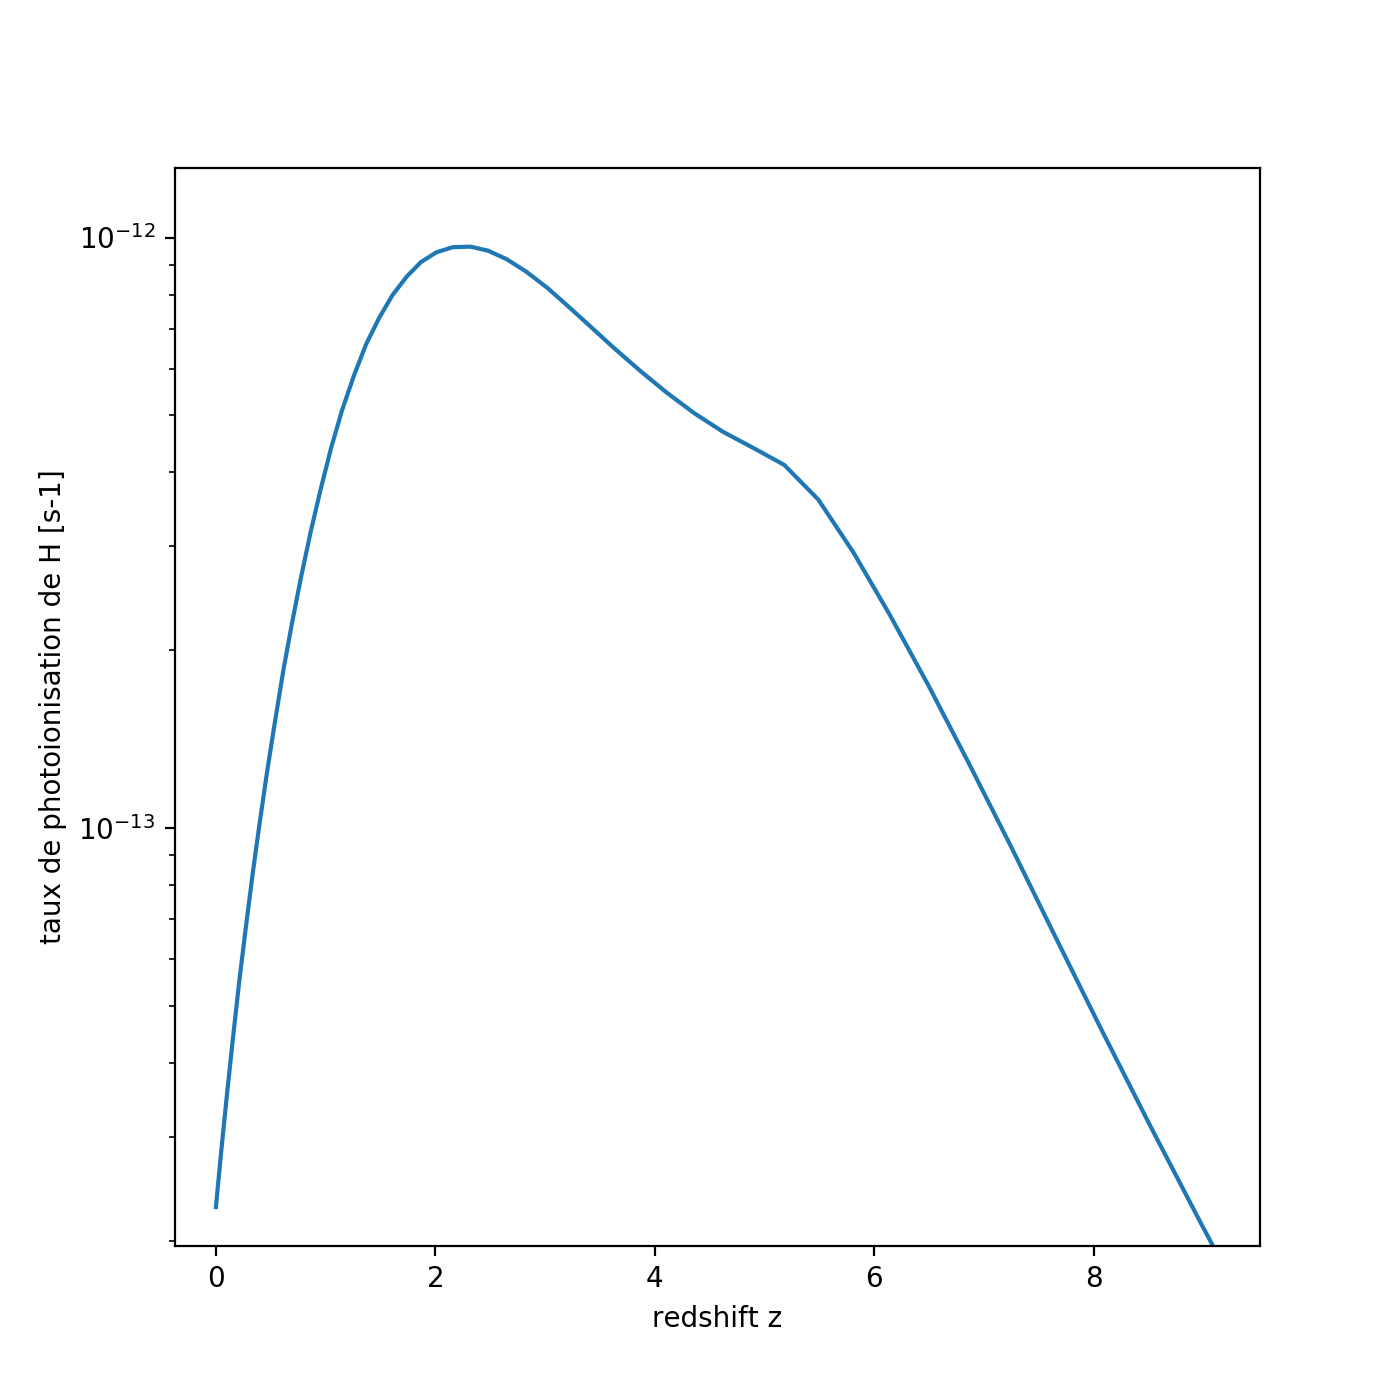
\includegraphics[height=12cm]{figs/HM.png}
	\caption[modèle de Haardt \& Madau]{Évolution en redshift du taux de photoionisations créées par le fond ultra-violet du modèle de Haardt \& Madau. Ce modèle suppose un Univers optiquement mince et sort de son domaine d'hypothèse pour z>6, lorsque l'Univers n'est pas complètement réionisé. On note une augmentation suivie d'une baisse du taux de photoionisation qui trace l'histoire cosmique de formation d'étoile.}
	\label{f:HM}
\end{figure}


\section{Formation et rétroaction stellaire}
L'objectif des simulations cosmologiques est d'explorer le processus de croissance des structures dans ses régimes les plus non linéaires et l'un des aboutissements de ces régimes est la formation d'étoile\index{etoiles@étoiles!formation}. Par ailleurs, la comparaison entre résultats de modélisation et observations se fait invariablement par la composante lumineuse des galaxies et à ce titre l'inclusion de modèles de formation stellaire est indispensable pour pouvoir comparer une vraie galaxie avec la composante stellaire d'une galaxie simulée.

\newthought{La résolution spatiale}\index{simulations numérique!résolution} nécessaire à modéliser la formation stellaire est néanmoins difficilement compatible avec les échelles cosmologiques. La formation stellaire opère dans des nuages moléculaires géants\index{nuage moléculaire}, aux tailles caractéristiques de l'ordre du parsec, tandis que les effets cosmologiques qui nous intéressent se manifestent sur des échelles supérieures au Mégaparsec : le rapport d'échelle est très important et à vrai dire hors de portée des machines actuelles de calcul. En effet, une haute résolution spatiale dans un grand volume cosmologique implique un grand nombre d'éléments de calculs (particules, cellules) et donc un grand nombre de données à traiter sur une très grande durée. Par exemple, un volume de 100 Mpc traité avec des cellules au parsec de résolution implique un nombre de cellules total de l'ordre de $(10^8)^3=10^{24}$. En 2017, les plus grandes simulations cosmologiques produites sur les plus grands calculateurs mondiaux traitent avec difficulté de problèmes échantillonnés sur $10^{11-12}$ cellules, bien en deçà de l'exigence que nous venons de formuler.

\newthought{La formation stellaire}\index{etoiles@étoiles!formation} ne peut donc être simulée à partir de «principes premiers»\sidenote{dans des volumes cosmologiques. Il existe des simulations à l'échelle du nuage moléculaires qui ont la résolution suffisante, mais qui se restreignent à des volumes physiques simulés bien insuffisants pour faire de la cosmologie.} et il faut donc avoir recours à des modèles. Une des approches les plus communes repose sur l'idée que la formation stellaire est régie par l'effondrement gravitationnel du gaz et opère donc sur des temps dynamiques\index{temps!dynamique} \sidenote{$\rho_*$ désigne la densité de masse stellaire formée, $\rho_g$ désigne la densité de gaz convertie en étoile et $t_g$ est le temps dynamique gravitationnel}:
\begin{equation}
\frac{d \rho_*}{dt}=\frac{d \rho_g}{dt}\sim\epsilon\frac{\rho_g}{t_g}.
\end{equation}
Ici $\epsilon$ désigne l'efficacité de formation stellaire et manifeste le fait que le temps caractéristique de formation d'étoile n'est pas exactement le temps dynamique, mais plutôt $t_g/\epsilon$ : l'efficacité est un paramètre libre du modèle.

Or le temps dynamique\index{temps!dynamique} est lui-même dépendant de la densité de gaz en effondrement:
\begin{equation}
t_g\sim\frac{1}{\sqrt{G\rho_g}}.
\end{equation}
Le taux de formation stellaire\index{taux de formation stellaire} (SFR \sidenote{de l'anglais \textit{Star Formation Rate}}) est alors décrit par une loi de puissance sur la densité de gaz présente localement:
\begin{equation}
\mathrm{SFR}\sim \epsilon \rho_g^{3/2}.
\label{e:schmidt}
\end{equation}
Cette relation est appelée \textit{Loi de Schmidt}\index{loi de Schmidt} et traduit en des termes simples qu'une région dense et riche en gaz produit naturellement plus d'étoiles : l'efficacité du processus est contrôlée par $\epsilon$ et opère sur des échelles de temps $t_g/\epsilon$. Observationnellement, on constate toutefois que le processus de formation stellaire est hautement inefficace avec des temps caractéristiques de conversion de l'ordre de quelques milliards d'années alors que les temps d'effondrement attendus sont environ 100 fois plus courts. L'efficacité de formation stellaire\index{efficacité de formation stellaire} est donc de l'ordre de $1\%$ et traduit l'impact macroscopique de processus non résolus qui empêche une formation d'étoile soutenue\sidenote{on ne connaît pas bien la source précise de cette inefficacité. Champs magnétiques, turbulence, vents stellaires sont souvent invoqués sans que leurs rôles relatifs et quantitatifs soient exactement connus.}.

\newthought{En pratique}, un code de simulation va passer en revue tous ses éléments de résolution et convertir une partie du gaz conformément à la Loi de Schmidt\index{loi de Schmidt}. Cette conversion va se manifester sous la forme de création de particules stellaires : ces particules n'interagissent que via la gravitation et se découplent du gaz comme de vraies étoiles. Ces «étoiles» possèdent un âge, éventuellement une composition chimique synthétique qui permet de leur assigner une luminosité ou un spectre pouvant amener des comparaisons entre ces populations stellaires simulées et celles observées dans les vraies galaxies. Rappelons pour finir que ces particules stellaires ont des masses typiques de l'ordre de 1000 $M_\odot$ à quelques millions et représentent donc des amas ou des populations stellaires et non pas des étoiles individuelles : nos machines actuelles ne sont pas capables de gérer le nombre réel d'étoiles présentes dans un volume cosmologique et doivent donc les regrouper en «macro-étoiles».

\newthought{Une étoile meurt}, parfois de façon spectaculaire si elle est massive, de l'ordre de la dizaine de masses solaire ou plus. Cette mort s'accompagne d'une explosion en supernova\index{supernova} qui va injecter de l'énergie dans le gaz environnant, le chauffer et donc prévenir au moins momentanément l'apparition de générations ultérieures d'étoiles (voir Fig. \ref{f:SN}). Une population existante va donc modérer l'apparition de populations suivantes dans un mécanisme de rétroaction\index{rétroaction}\sidenote{en anglais on parle aussi de \textit{feedback}}. Les codes de simulations vont modéliser cette rétroaction en injectant de l'énergie dans le gaz à proximité des particules stellaires qui atteignent l'âge correspondant à l'apparition des premières explosions. Notons que toute la population stellaire d'une particule stellaire n'est pas concernée : une population contient des étoiles massives, qui explosent, et des étoiles légères de type solaire qui ont des durées de vie de l'ordre de l'âge de l'Univers. La répartition des masses au sein d'une population est donnée par la \textit{fonction de masse initiale}\index{fonction de masse initiale}. Observationnellement cette répartition est souvent décrite par une \textit{loi de Salpeter}\index{loi de Salpeter} dans un grand nombre de contextes \sidenote{$N(m)$ désigne le nombre d'étoiles de masse $m$ à $dm$ près}:
\begin{equation}
N(m)dm\sim m^{-2.35}dm
\end{equation}
qui traduit le fait qu'une population naissante possède un grand nombre d'étoiles de faible masse et un nombre plus faible d'étoiles massives susceptibles de réinjecter de l'énergie dans le gaz environnant. Cette fonction de masse initiale, comme toutes les autres, permet de contraindre la fraction d'étoiles qui vont exploser ainsi que la répartition temporelle (durée, instant) de cette réinjection d'énergie.

\begin{figure}[htbp]
	\centering
		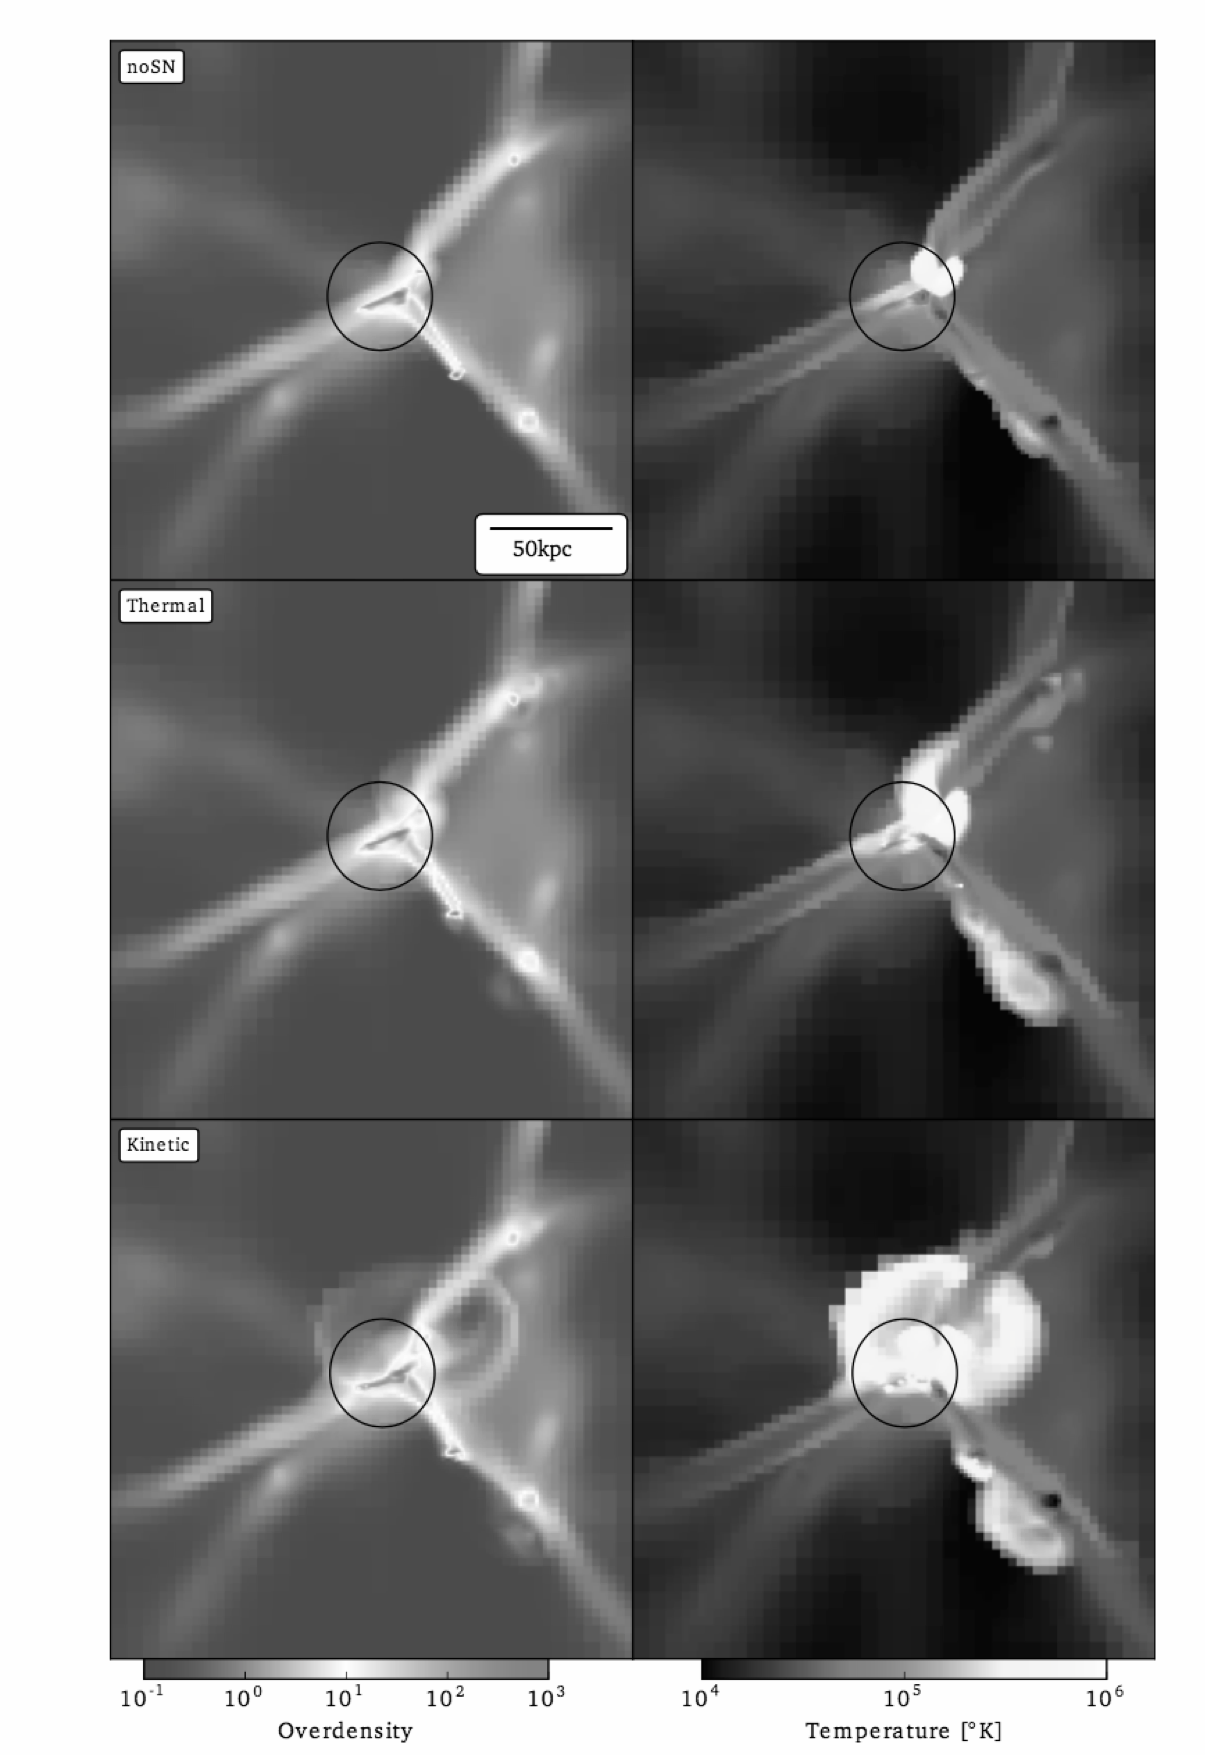
\includegraphics[height=13cm]{figs/SN.png}
	\caption[Exemples d'injection d'énergie par une particule stellaire modélisant l'explosion d'une supernova. ]{Exemples d'injection d'énergie par une particule stellaire modélisant l'explosion d'une supernova. La colonne de gauche montre la densité de gaz autour d'une galaxie pesant $1/10$ème de la masse de la Voie Lactée. La colonne de droite montre la température du gaz. La ligne supérieure montre une simulation sans explosion tandis que les 2 lignes inférieures montrent 2 modèles d'explosion. On note la montée en température du gaz lors de la présence d'explosion ainsi que la création de fronts produits par le gaz expulsé.}
	\label{f:SN}
\end{figure}

\newthought{Les trous noirs supermassifs}\index{trou noir!supermassif} ont aussi un rôle à jouer dans ces modèles à base de simulation. Ils sont en effet les moteurs des \textit{noyaux actifs de galaxies}\index{noyau actif de galaxie}, les AGNs \sidenote{pour \textit{active galactic nuclei}}, qui renvoient dans les galaxies plus massives et leur proche environnement une partie de l'énergie acquise par l'accrétion de matière par le trou noir central. Le taux d'accrétion d'un trou noir de masse $M_\bullet$ est souvent approximé par la formule d'accrétion de Bondi\index{accrétion de Bondi}
\begin{equation}
M_\mathrm{Bondi}\sim \pi \rho v R_s^2.
\end{equation}
Cette formule est une approximation simple du taux d'accrétion autour d'un trou noir se déplaçant à une vitesse $v$ dans un milieu de densité $\rho$ : l'accrétion se fait au travers d'une surface de rayon $R_s=2GM_\bullet/c_s^2$ \sidenote{c'est tout simplement la distance où la vitesse de libération est égale à celle du son}, qui est la distance où la vitesse du son $c_s$ du milieu environnant n'est pas suffisante pour s'opposer à l'attraction. Des particules «trous noirs» sont ainsi parfois ajoutées dans les simulations cosmologiques et dont la masse va grandir sous l'effet de l'accrétion de matériau pour atteindre parfois des masses de l'ordre du million de masses solaires. Une partie de l'énergie ainsi accumulée va être réinjectée dans le gaz environnant, produisant un effet similaire à la rétroaction des supernovæ créées par les étoiles :
\begin{equation}
E_{\mathrm{TN}}=\epsilon M_\mathrm{Bondi} c^2.
\end{equation}
Contrairement aux étoiles, cette accrétion, et donc cette injection d'énergie, dépend des conditions locales d'accrétion. Ce type de rétroaction est nécessaire pour expliquer par exemple l'abondance des galaxies brillantes, qui est plutôt plus faible que celle attendue par une simple extrapolation du nombre de halos de matière noire\index{halo de matière noire}\sidenote{voir le chapitre dédié à la matière noire} très massifs : l'énergie produite par les AGNs, par effet thermique ou mécanique, réduit l'efficacité de formation stellaire dans ces objets.

\newthought{Tous ces modèles sous-grilles} sont susceptibles de multiples variations dans toutes les étapes, traduisant notre manque de connaissance actuel sur les processus à l'œuvre autour de la formation stellaire ou bien la vue nécessairement grossière de phénomènes fins vus depuis les échelles cosmologiques. Par conséquent, les simulations, qui visent à reproduire l'Univers et les galaxies observées, disposent de multiples leviers sur lesquels agir et qui constituent autant de paramètres libres. Par ailleurs, on sait que d'autres physiques sous-estimées ou non modélisées ont peut-être leur rôle à jouer et de fait tout accord entre simulations et observations peut être critiqué\sidenote{comme étant dépendant de l'expérience réalisée ou accidentel par exemple} et tout désaccord peut être minimisé en invoquant une physique mal ou non résolue. La section dédiée à la matière noire survole les quelques problèmes rencontrés par les prédictions numériques : ces problèmes sont la conséquence du caractère beaucoup plus complexe, plus non linéaire et multiforme des physiques en jeu lorsque l'on quitte le domaine de la cosmologie à proprement dit pour aborder celui de la formation des galaxies. Il n'en reste pas moins que les simulations sont les seuls outils de modélisation nous permettant d'étudier ces processus dans leur plus grande complexité.
